\section{Argument Schemes for Goal Modeling (GMAS)}
\label{sect:gmas}

In this section, we develop a set of argument schemes and critical questions for goal modeling. The final list of argument schemes and critical questions is shown in Table~\ref{table:argument-schemes}. The first four argument schemes (AS0-AS4) are argument for an element of a goal model, the next seven (AS5-AS11) are about relationships, the next two (AS12-AS13) are about intentional elements in general, and the last is (Att) is a generic counterargument for any type of argument that has been put forward. For each critical question, the right column shows the effect of answering the critical questions affirmatively, which can be \textsf{DISABLE} (disable the element of the original argument), \textsf{INTRO} (introduce a new element and argument), \textsf{REPLACE} (replace the element of the original argument), \textsf{ATTACK} (attack an argument directly). For instance, if the critical question CQ0 ``Is the actor relevant?'' is answered with ``No'', then the actor of the original argument AS0 will be disabled in the goal model.

%SG: If we only obtained them from these transcripts, how can we be sure that they are complete or even sufficient? Also, what are the transcripts? where did you take them from? why are they useful and why are they relevant?
We obtained the list in Table~\ref{table:argument-schemes} by analyzing transcripts of discussions between students about the development of an information system. In the first subsection, we provide details of this analysis process with concrete examples, after which we analyze our results in the next subsection. In the last subsection, we provide several examples of the effect of answering a critical question. In the next section, we develop a formal language for our argument schemes, critical questions, and the effect of answering them.

%SG: some comments on the table: softgoals can't decompose into goals or tasks? tasks don't contribute to goals? tasks mainly depend on resources.. why do we have A6 and A11? Note that GRL doesn't have those restrictions some languages such as i* have.. for example a softgoal can technically contribute to a task or a task can be decompsosed into goals.. how do you address those? We also mentioned in background that this is the benefit of GRL over i* so why do we now don't address it?

\begin{table*}[h]
\centering
\begin{tabularx}{\textwidth}{|l|l|l|X|l|l|}
\hline
\multicolumn{2}{|c|}{\textbf{Argument scheme}} & \multicolumn{2}{c|}{\textbf{Critical Questions}} & \textbf{Effect}\\
\hline
AS0 & Actor $a$ is relevant & CQ0 &Is the actor relevant? & DISABLE\\
\hline
AS1 & Actor $a$ has resource $R$ & CQ1 &Is the resource available? & DISABLE\\
\hline
AS2 & Actor $a$ can perform task $T$ & CQ2 &Is the task possible? & DISABLE\\
\hline
AS3 & Actor $a$ has goal $G$ & CQ3 & Can the desired goal be realized? & DISABLE\\
\hline
AS4 & Actor $a$ has softgoal $S$ & CQ4 & Is the softgoal a legitimate softgoal?& DISABLE\\
\hline
\hline
AS5 & Goal $G$ decomposes into tasks $T_1,\ldots,T_n$ & CQ5a & Does the goal decompose into the tasks?& DISABLE\\
& & CQ5b & Does the goal decompose into any other tasks?& REPLACE\\
\hline
AS6 & Task $T$ contributes to softgoal $S$& CQ6a & Does the task contribute to the softgoal?& DISABLE\\
&& CQ6b & Are there alternative ways of contributing to the same softgoal?& INTRO \\
&& CQ6c & Does the task have a side effect which contribute negatively to some other softgoal?& INTRO\\
&& CQ6d & Does the task contribute to some other softgoal?& INTRO\\
\hline
AS7 & Goal $G$ contributes to softgoal $S$ & CQ7a & Does the goal contribute to the softgoal?& DISABLE\\
&& CQ7b & Does the goal contribute to some other softgoal?& INTRO\\
\hline
AS8 & Resource $R$ contributes to task $T$ & CQ8 & Is the resource required in order to perform the task?& DISABLE\\
\hline
AS9 & Actor $a$ depends on actor $b$ & CQ9 & Does the actor depend on any actors?& INTRO\\
\hline
AS10 & Task $T_1$ decomposes into tasks $T_2,\ldots,T_n$ & CQ10a & Does the task decompose into other tasks?& REPLACE\\
 &  & CQ10b & Is the decomposition type correct? (AND/OR/XOR)& REPLACE\\
\hline
AS11 & Task $T$ contributes negatively to softgoal $S$& CQ11 & Does the task contribute negatively to the softgoal?& DISABLE\\
\hline
\hline
AS12 & Element $IE$ is relevant & CQ12 & Is the element relevant/useful? & DISABLE\\
\hline
AS13 & Element $IE$ has name $n$ & CQ13 & Is the name clear/unambiguous? & REPLACE\\
\hline
\hline
- & - & Att & Generic counterargument & ATTACK\\
\hline
\end{tabularx}
\caption{List of argument schemes (AS0-AS13, left column), critical questions (CQ0-CQ12, middle column), and the effect of answering them (right column).}
\label{table:argument-schemes}
\end{table*}

\subsection{Details experiment}

The transcripts we used are created as part of two master theses on improving design reasoning~\cite{masterthesis1,masterthesis2}.

\paragraph{Subjects} The subjects for the case study are three teams of Master students from the University of Utrecht, following a Software Architecture course. Two teams consist of three students, and one team consists of two students.

\paragraph{Experimental Setup} The assignment used for the experiments is to design a traffic simulator. Designers are provided a problem description, requirements, and a description of the desired outcomes. The original version of the problem descrption~\cite{UCIworkshop} is well known in the field of design reasoning since it has been used in a workshop\footnote{\url{http://www.ics.uci.edu/design-workshop/}}, and transcripts of this workshop have been analyzed in detail~\cite{Petre:2013:SDA:2535028}. Although the concepts of traffic lights, lanes, and intersections are common and appear to be simple, building a traffic simulator to represent these relationships and events in real time turns out to be challenging. Participants were asked to use a think-aloud method during the design session. The assignment was slightly adjusted to include several viewpoints as end products in order to conform to the course material~\cite{Bass:2012:SAP:2392670}. The final problem descriptions can be found in Appendix A of Schriek's master thesis~\cite{masterthesis1}. All groups were instructed to apply the \emph{functional architecture method}, focusing on developing the \emph{context}, the \emph{functional}, and the \emph{informational} viewpoints of the traffic simulator software. The students had two hours for the tasks, and the transcripts document the entire discussion. The details of the transcripts are shown in table~\ref{table:transcripts:info}.

\begin{table}[ht]
\centering
\begin{tabular}{|l|l|l|l|}
\hline
& transcript $t_1$ & transcript $t_2$ & transcript $t_3$\\
\hline
participants & 2 & 3 & 3\\
\hline
duration & 1h34m52s & 1h13m39s & 1h17m20s\\
\hline
\end{tabular}
\caption{Number of participants and duration of the transcripts.}
\label{table:transcripts:info}
\end{table}

\paragraph{Annotation Method} 

%SG: here we say we started from pras and then added more questions.. in the first paragraph we say the questions are coming from the transcripts!This is better... and we should mention it above..
We started with an initial list of 10 argument schemes and 18 critical questions that we derived from PRAS. We annotated transcripts with the arguments and critical questions from this list. If we found arguments or critical questions that did not appear in the original list, we added them and counted them as well. Argument schemes that did not appear were removed from the list, but critical questions were not removed (see discussion in Section~\ref{sect:gmas:transcripts:analysis}). Most of the occurrences were not literally found back, but had to be inferred from the context. This can be seen in the various examples we will discuss.

\todo{Marc}{Floris}{I'd like to say something in the next paragraph about the difficulty of extracting arguments from text. Do you know any references?}
It is generally known in the argumentation literature that it can be very difficult to annotate arguments correctly. Arguments are often imprecise, lack conclusion, and may be supported by non verbal communication that is not captured in the transcripts. Still, since research on argument extraction in the requirement engineering domains is in its infancy, we believe that our evaluation is useful by itself. Furthermore, our annotation is openly available\footnote{\todo{Marc}{Marc}{provide url}}, we provide parts of our annotation in Appendix~\ref{sect:transcripts:excerpts}, and most of the examples from this article come from the transcripts. In this way, we aim to make our annotation process as transparent as possible.

\paragraph{Results}

\begin{figure*}[h]
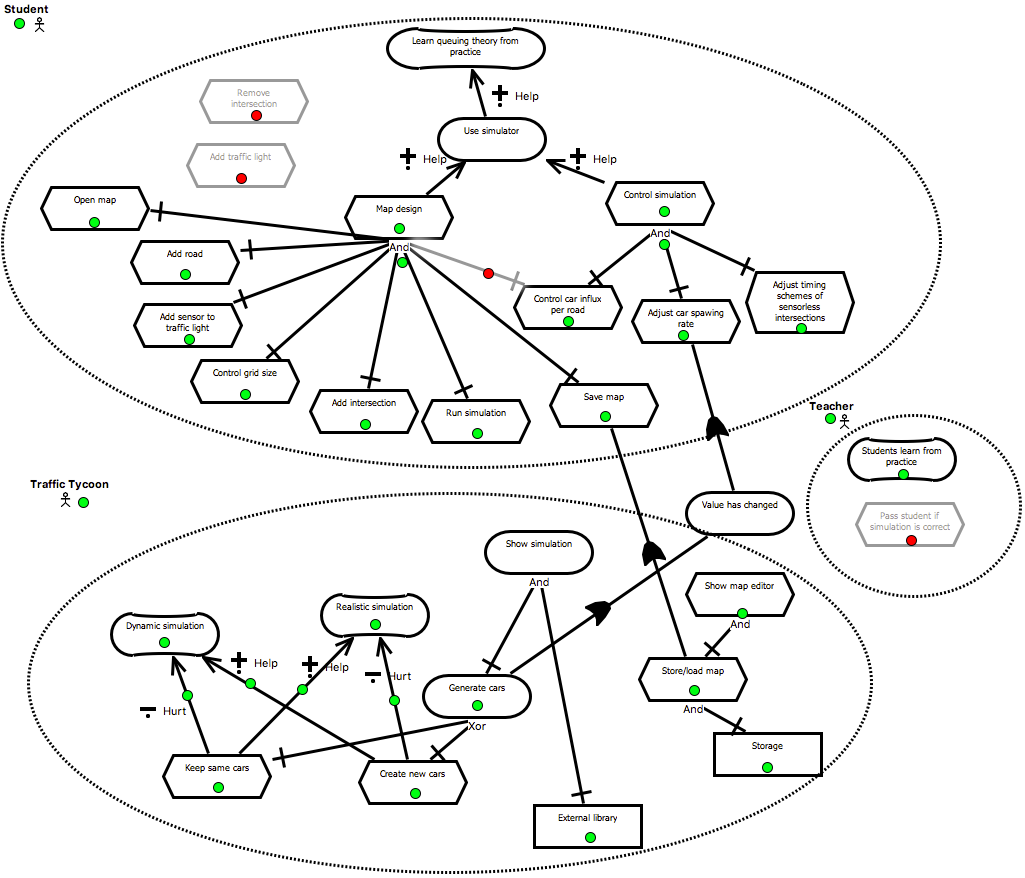
\includegraphics[width=\textwidth]{img/transcript_grl}
\caption{The GRL model manually constructed from transcript $t_1$. Green dots indicate accepted underlying arguments, red dots indicate rejected underlying arguments. Elements and relationships with no dot have been inferred by us.}
\label{fig:transcripts:grl}
\end{figure*}


We found a total of 159 instantiations of the argument schemes AS0-AS11 in the transcripts. The most used argument scheme was AS2: ``Actor $A$ has task $T$'', but each argument scheme has been found back in the transcripts at least twice (Table~\ref{table:transcripts:results:argumentschemes}). A large portion (about 60\%) of the argument schemes we found involved discussions around tasks of the information system (AS2, AS10).

We annotated 41 applications of critical questions. Many critical questions (about 55\%) involved clarifying the name of an element, or discussing about the relevance of it (CQ12, CQ13).

\begin{table}[ht]
\centering
\begin{tabularx}{0.5\textwidth}{|l|X|l|l|l|>{\bfseries}l|}
\hline
\multicolumn{2}{|c|}{\textbf{Scheme/Question}} & $t_1$ & $t_2$ & $t_3$ & \textbf{total}\\
\hline 
AS0 & Actor & 2 & 2 & 5 & 9\\
\hline
AS1 & Resource & 2 & 4 & 5 & 11\\
\hline
AS2 & Task/action & 20 & 21 & 17 & 58\\
\hline
AS3 & Goal & 0 & 2 & 2 & 4\\
\hline
AS4 & Softgoal & 3 & 4 & 2 & 9\\
\hline
AS5 & Goal decomposes into tasks & 4 &0& 4 & 8\\
\hline
AS6 & Task contributes to softgoal & 6 & 2 &0& 8\\
\hline
AS7 & Goal contributes to softgoal &0& 1 & 1 & 2\\
\hline
AS8 & Resource contributes to task & 0 & 4 & 3 & 7\\
\hline
AS9 & Actor depends on actor &0& 1 & 3 & 4\\
\hline
AS10 & Task decomposes into tasks & 11 &14 &11 &36\\ 
\hline
AS11 & Task contributes negatively to softgoal & 2 & 1 & 0 & 3\\
\hline
\hline
CQ2 & Task is possible? & 2 & 2 & 1 & 5\\
\hline		
CQ5a & Does the goal decompose into the tasks? & 0 & 1 & 0 & 1\\
\hline
CQ5b & Goes decomposes into other tasks? & 1 & 0 & 0 & 1\\
\hline
CQ6b & Task has negative side effects? & 2 & 0 & 0 & 2\\
\hline
CQ10a & Task decompose into other tasks? & 1 &2 &0&3\\
\hline
CQ10b & Decomposition type correct? &1 &0& 1 &2\\
\hline
\hline
CQ12 & Is the element relevant/useful? & 2 & 3 & 2 &7\\
\hline
CQ13 & Is the name clear/unambiguous? &3 &10 & 3 & 16\\
\hline
\hline
- & Generic counterargument & 0& 2 & 2 & 4\\
\hline
\hline
\multicolumn{2}{|c|}{\textbf{TOTAL}}&69&80&69&222\\
\hline
\end{tabularx}
\caption{Number of occurrences of AS0-AS9, CQ0-CQ12 in the transcripts. Critical questions not appearing in this table were not found back in the transcripts.}
\label{table:transcripts:results:argumentschemes}
\end{table}

For each transcript, we manually create a GRL model from the argument schemes and critical questions we found in them, in order to verify whether the arguments put forward by the participants were sufficiently informative. An example of such a model is shown in Figure~\ref{fig:transcripts:grl}. We added green and red dots to various elements and relationships in the Figure. A green dot indicates there is an underlying argument for the element that is accepted, while a red dot indicates a rejected underlying argument. Note that if the underlying argument is rejected, the corresponding GRL element has been disabled. Some elements do not have a corresponding green or red dot. In that case, we have inferred the elements from the discussion, but we could not explicitly find back arguments for it.

We found that answering a critical questions can have four different effects on the original argument: \todo{Sepideh}{all}{Examples here are from the meeting scheduler! and our figure is about traffic simulator}
\begin{itemize}
\item \emph{INTRO}: Introduce a new goal element or relationship with a corresponding argument. This operation does not attack the original argument of the critical question, but rather creates a new argument. For instance, suppose argument scheme AS5 is instantiated as follows:: ``Goal \emph{Agreeable meeting dates} OR-decomposes into tasks \emph{Find agreeable date using scheduler} and \emph{Find agreeable date by talking to initiator}'' (Figure~\ref{fig:SchedulerModel}). Suppose now the critical question CQ5b: ``Does the goal \emph{Agreeable meeting dates} decompose into other tasks?'' is answered with ``yes, namely \emph{Find agreeable date by contacting secretary}''. This results in a new instantiation of AS5, namely: ``Goal \emph{Agreeable meeting dates} OR-decomposes into tasks \emph{Find agreeable date using scheduler}, \emph{Find agreeable date by talking to initiator}, and \emph{Find agreeable date by contacting secretary}. As a result, the goal model will contain the corresponding task \emph{Find agreeable date by contacting secretary}, as well as an OR-decomposition relation from the goal \emph{Agreeable meeting dates} to that task.
\item \emph{DISABLE:} Disable the element or relationship of the argument scheme to which the critical questions pertains. This operation does not create a new argument, but only disables (i.e., attacks) the original one. For instance, suppose argument scheme AS0 is instantiated with: ``Actor \emph{meeting initiator} is relevant'' (Figure~\ref{fig:SchedulerModel}). This argument can be attack with critical question CQ0: ``Actor \emph{meeting initiator} is not relevant''. As a result, the argument for the actor is attack, and actor \emph{meeting initiator} is disabled in the goal model.
\item \emph{REPLACE:} Replace the element of the argument scheme with a new element. This operation both introduces a new argument and attacks the original one. For instance, suppose argument scheme AS2 is instantiated wit: ``Actor \emph{meeting initiator} can perform task \emph{schedule meeting}. This argument can be attacked with critical question CQ13: ``The task \emph{schedule meeting} is unclear, it should be \emph{schedule board meeting}''. This results in replacing the original argument with the new argument ``Actor \emph{meeting initiator} can perform task \emph{schedule board meeting}. In the goal model, the description of the task should change accordingly.
\item \emph{ATTACK:} Attack any argument with an argument that cannot be classified as a critical question. For instance, suppose argument scheme AS4 is instantiated as follows: ``Actor \emph{meeting initiator} has goal \emph{quick}. For instance, suppose argument scheme AS0 is instantiated with ``Actor \emph{meeting scheduler} is relevant''. Suppose this argument is attacked with critical question CQ0: ``Actor \emph{meeting initiator} is not relevant'', because the participants decide to fully automate the meeting scheduling process. However, this critical question may in turn be attacked again, if new evidence comes up. For instance, it may turn out that it is sometimes more desirable to schedule meeting by hand. In this case, the generic counter argument ``Actor \emph{meeting initiator} is relevant, because it is sometimes easier to schedule meetings manually'' attack the argument ``Actor \emph{meeting scheduler} is not relevant''. As a result, the original argument ``Actor \emph{meeting scheduler} is relevant'' is accepted again, and as a result is shown in the goal model.
\end{itemize}

In Section~\ref{sect:gmas:examples} we provide examples we found in the transcripts for all of these four effects.

\subsection{Analysis}
\label{sect:gmas:transcripts:analysis}

\paragraph{Analysis of the Argument Schemes}
Our initial list of argument schemes consists of AS1-AS4, AS5-AS9 (Table~\ref{table:argument-schemes}). Therefore, the difference between the initial list of argument schemes and those found back in the transcripts is quite small. We found it surprising that we were able to find back all the schemes in the transcript at least twice, even more since the topic of discussion was not goal models, but more generally the architecture of an information system. This gives us an indication that these argument schemes are able to capture arguments used in those type of discussions to some extent. 

More generally, we observed that our initial list is rather limited, which is a consequence of the fact that it is derived from PRAS. Since PRAS only considers very specific types of relationships, we are not able to capture many other relationships existing in GRL. GRL has four types of intentional elements (softgoal, goal, task, resource) and four types of relationships (positive contribution, negative contribution\footnote{In fact, a contribution can be any integer in the domain [-100,100], but for the sake of simplicity we only consider two kinds of contributions here.}, dependency, decomposition), allowing theoretically $4^3=64$ different types of argument schemes, of which we currently only consider 11. Our analysis however shows that many of these schemes are not often used, and thus, gives us some confidence in the resulting list. \todo{Sepideh}{all}{how does the analysis show that? also, what if someone says that you mentioned above that the transcripts were not used for goal models and that is why you didn't have those schemes.. what if someone is doing arguments for goal models, how do you make sure that the list is good enough, especially that many of the relationships are not considered?)}

\paragraph{Analysis of the Critical Questions} The difference between the initial list of critical questions and those we found back in the transcripts is much larger than for the critical questions. %SG: I don't get this sentence. Also, the ones below. 
On the one hand, we found a few of the critical questions we initially proposed. However, this does not mean that they were not implicitly used in the minds of the participants. If a participants makes an argument for a contribution from a task to a softgoal, it may very well be that she was asking herself the question ``Does the task contribute to some other softgoal?''. However, many of these critical questions are not mentioned explicitly. If we assume this explanation is at least partially correct, then, this would mean that critical questions may still play a role when formalizing the discussions leading up to a goal model, and it would be limiting to leave them out of our framework. In the context of tool support, we believe that having these critical questions available may stimulate discussions.

\subsection{Examples}
\label{sect:gmas:examples}

We now discuss various instantiations of argument schemes and the result of answering critical questions in more detail. For each example we provide transcript excerpts, a visualization of the arguments, and the corresponding goal model elements. We provide a legend for our visualization notation in Figure~\ref{fig:legend}.

\begin{figure}[ht!]
\centering
\begin{tikzpicture}
        \node (att1) [argNodeIN] at (-5,0) {$A_1$};
        \node (att2) [argNodeOUT] at (-2,0) {$A_2$};
        \node (attDescription) [draw=none, align=center] at (0.5,0) {Argument $A_1$ (accepted)\\ attacks argument $A_2$\\ (rejected)};
        \node[traceNodeGREEN] (trace1a) at (-5,-1.5) {};
        \node[traceNodeGREEN] (trace1b) at (-2,-1.5) {};
        \node (traceDescription) [draw=none,align=center] at (0.5,-1.5) {Traceability link from\\ accepted argument to\\ enabled GRL element};
        \node[traceNodeRED] (trace2a) at (-5,-3) {};
        \node[traceNodeRED] (trace2b) at (-2,-3) {};
        \node (traceDescription) [draw=none,align=center] at (0.5,-3) {Traceability link from\\ rejected argument to\\ disabled GRL element};
        \node (cq1) [argNodeIN] at (-5,-4.5) {$A_1$};
        \node (cq2) [argNodeIN] at (-2,-4.5) {$A_2$};
        \node (cqDescription) [draw=none,align=center] at (0.5,-4.5) {Argument $A_2$ is the result of\\ answering critical question\\ $CQ$ of argument $A_1$};
         \path
    (att1) edge [attackLink] (att2)
    (cq1) edge [CQLink] node [above,draw=none] {CQ} (cq2)
    (trace1a) edge[traceLinkGREEN] (trace1b)
    (trace2a) edge[traceLinkRED] (trace2b);
\end{tikzpicture}
\caption{Legend of the various elements and relationships we use for the examples in this article.}
\label{fig:legend}
\end{figure}


\subsubsection{Example 1: Disable task \emph{Traffic light}}

The transcript excerpt of this example is shown in Table~\ref{table:transcripts:traffic-light} in the Appendix and comes from transcript $t_1$. In this example, participants are summing up functionality of the traffic simulator, which are tasks that the student can perform in the simulator. All these task can be formalized and are instantiations of argument scheme AS2: ``Actor \emph{Student} has tasks $T$'', where $T\in\{$Save map, Open map, Add intersection, Remove intersection, Add road, Add traffic light$\}$''. 

Once all these tasks are summed up, participant \texttt{P1} notes that the problem description states that all intersections in the traffic simulator have traffic lights, so the task \texttt{Add traffic light} is not useful. We formalized this using the critical question CQ12: ``Is task \texttt{Add traffic light} useful/relevant?''.

We visualize some of the argument schemes, critical questions, and traceability links with the GRL model in Figure~\ref{fig:examples:traffic-light}. On the left side of the image, we see three of the instantiated argument schemes AS2. The bottom one, ``Actor \texttt{Student} has task \texttt{Add traffic light}'', is attacked by another argument generated from applying critical question CQ12: ``\texttt{Add traffic light} is useless (\emph{All intersections have traffic lights}). As a result, the corresponding GRL task is disabled. The other two tasks are enabled and have green traceability links.

\begin{figure}[ht!]
\centering
        \begin{tikzpicture}
        \node (a0) [argNodeIN] at (-2,0) {
        	\argtext{AS2}{Actor \emph{Student} has task \emph{Save map}}
        };
        \node (a1) [argNodeIN] at (-2,-2) {
        	\argtext{AS2}{Actor \emph{Student} has task \emph{Add road}}
        };
        \node (a2) [argNodeOUT] at (-2,-4) {
        	\argtext{AS2}{Actor \emph{Student} has task \emph{Add traffic light}}
        };
        \node (a3) [argNodeIN] at (-2,-6){
        	\argtext{}{\emph{Add traffic light} is useless (\emph{All intersections have traffic lights})}
        };
        \node[grl] (task1) at (2.3,0) { 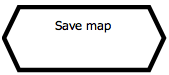
\includegraphics[scale=0.5]{img/task_save_map} };
        \node[grl] (task2) at (2.3,-2) { 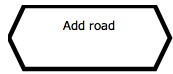
\includegraphics[scale=0.5]{img/task_add_road} };
        \node[grl, disabled] (task3) at (2.3,-4) { 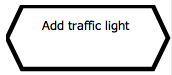
\includegraphics[scale=0.5]{img/task_add_traffic_light} };
        \node[traceNodeGREEN] (trace1a) at (-.4,-.3) {};
        \node[traceNodeGREEN] (trace1b) at (2.2,-.3) {};
        \node[traceNodeGREEN] (trace2a) at (-.4,-2.3) {};
        \node[traceNodeGREEN] (trace2b) at (2.2,-2.3) {};
        \node[traceNodeRED] (trace3a) at (-.4,-4.3) {};
        \node[traceNodeRED] (trace3b) at (2.2,-4.3) {};
         \path
    (a3) edge [attackLink] (a2)
    (a2) edge [CQLink, bend right=50] node [left,draw=none] {CQ12} (a3)
    (trace1a) edge[traceLinkGREEN] (trace1b)
    (trace2a) edge[traceLinkGREEN] (trace2b)
    (trace3a) edge[traceLinkRED] (trace3b);
\end{tikzpicture}
\caption{Argument schemes and critical questions (left), GRL model (right), and traceability link (dotted lines) for the traffic light example.}
\label{fig:examples:traffic-light}
\end{figure}


\subsubsection{Example 2: Clarify task \emph{Road pattern}}

The transcript excerpt of the second example is shown in Table~\ref{table:transcript:task-clarification} in the Appendix and comes from transcript $t_3$. It consists of a number of clarification steps, resulting in the task \texttt{Choose a road pattern}. 

\begin{figure}[ht!]
\centering
        \begin{tikzpicture}[->]
        \node (a0) [argNodeOUT] at (-2,0) {
        	\argtext{AS2}{Actor \emph{Student} has task \emph{Create road}}
        };
        \node (a1) [argNodeOUT] at (-2,-2) {
        	\argtext{AS2}{Actor \emph{Student} has task \emph{Choose a pattern}}
        };
        \node (a2) [argNodeOUT] at (-2,-4.2) {
        	\argtext{AS2}{Actor \emph{Student} has task \emph{Choose a pattern preference}}
        };
        \node (a3) [argNodeIN] at (-2,-6.7) {
        	\argtext{AS2}{Actor \emph{Student} has task \emph{Choose a road pattern}}
        };
        \node[grl] (actor) at (2.3,-4) { 
        	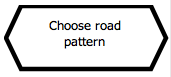
\includegraphics[scale=0.5]{img/task_choose_road_pattern} 
        };
        \node[traceNodeGREEN] (trace1) at (-.5,-7.1) {};
        \node[traceNodeGREEN] (trace2) at (2.2,-4.4) {};

\begin{pgfonlayer}{background}
         \path
    (a1) edge[attackLink] (a0)
    (a2) edge[attackLink] (a1)
    (a2) edge[attackLink, bend right=20] (a0)
    (a3) edge[attackLink] (a2)
    (a3) edge[attackLink, bend right=20] (a1)
    (a3) edge[attackLink, bend right=40] (a0);
\end{pgfonlayer}

	\path
	(a0) edge [CQLink, bend right=50] node [left,draw=none] {CQ12a} (a1)
    (a1) edge [CQLink, bend right=50] node [left,draw=none] {CQ12a} (a2)
    (a2) edge [CQLink, bend right=50] node [left,draw=none] {CQ12a} (a3)
    (trace1) edge[traceLinkGREEN] (trace2);
\end{tikzpicture}
\caption{Argument schemes and critical questions (left), GRL model (right), and traceability link (dotted line) of the road pattern example.}
\label{fig:examples:clarification}
\end{figure}

The formalized argument schemes and critical questions are shown in Figure~\ref{fig:examples:clarification}. The discussion starts with the first instantiation of argument scheme AS2: ``Actor \texttt{Student} has task \texttt{Create road}''. This argument is then challenged with critical question CQ12: ``Is the task \texttt{Create road} clear?''. Answering this question results in a new instantiation of argument scheme AS2: ``Actor \texttt{Student} has task \texttt{Choose a pattern}''. This process is repeated two more times, resulting in the final argument ``Actor \texttt{Student} has task \texttt{Choose a road pattern}''. This final argument is unattacked and has a corresponding intentional element (right image). 

What is clearly shown in this example is that a clarifying argument attacks all arguments previously used to describe the element. For instance, the final argument on the bottom of Figure~\ref{fig:examples:clarification} attacks all previous arguments. If this was not the case, then it may occur that a previous argument is \emph{reinstatiated}, meaning that it becomes accepted again because the argument attacking it is itself attacked.

\subsubsection{Example 3: Decompose goal \emph{Simulate}}

The transcript excerpt of this example is shown in Table~\ref{table:transcript:decomposition} in the Appendix and comes from transcript $t_3$. It consists of a discussion about the type of decomposition relationship for the goal \texttt{Simulate}.

\begin{figure}[ht!]
\centering
        \begin{tikzpicture}[->]
        \node (a0) [argNodeIN] at (-2,0) {
        	\argtext{AS3}{Actor \emph{System} has goal \emph{Simulate}}
        };
        \node (a1) [argNodeIN] at (-2,-1.5) {
        	\argtext{AS2}{Actor \emph{System} has task \emph{Dynamic simulation}}
        };
        \node (a2) [argNodeIN] at (-2,-3) {
        	\argtext{AS2}{Actor \emph{System} has task \emph{Static simulation}}
        };
        \node (a3) [argNodeOUT] at (-2,-5) {
        	\argtext{AS5}{Goal \emph{Simulate} AND-decomposes into \emph{Static simulation} and \emph{Dynamic simulation}}
        };
        \node (a4) [argNodeIN] at (-2,-7.5) {
        	\argtext{AS5}{Goal \emph{Simulate} OR-decomposes into \emph{Static simulation} and \emph{Dynamic simulation}}
        };
        \node[grl] (actor) at (2.3,-4) { 
        	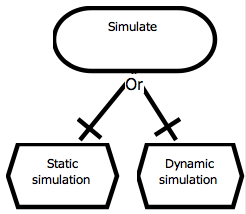
\includegraphics[scale=0.5]{img/simulate_decomposition} 
        };
        \node[traceNodeGREEN] (trace1a) at (-.4,-.3) {};
        \node[traceNodeGREEN] (trace1b) at (2.5,-3.1) {};
        \node[traceNodeGREEN] (trace2a) at (-.4,-1.8) {};
        \node[traceNodeGREEN] (trace2b) at (3.5,-5.6) {};
        \node[traceNodeGREEN] (trace3a) at (-.4,-3.3) {};
        \node[traceNodeGREEN] (trace3b) at (1.3,-5.6) {};
        \node[traceNodeGREEN] (trace4a) at (-.4,-8.2) {};
        \node[traceNodeGREEN] (trace4b) at (2.5,-3.9) {};

\begin{pgfonlayer}{background}
         \path
    (a4) edge[attackLink] (a3);
\end{pgfonlayer}

	\path
	(a3) edge [CQLink, bend right=50] node [left,draw=none] {CQ10b} (a4)
    (trace1a) edge[traceLinkGREEN] (trace1b)
    (trace2a) edge[traceLinkGREEN] (trace2b)
    (trace3a) edge[traceLinkGREEN] (trace3b)
    (trace4a) edge[traceLinkGREEN, bend right] (trace4b);
\end{tikzpicture}
\caption{Argument schemes and critical questions (left), GRL model (right), and traceability link (dotted line) of the goal decomposition example.}
\label{fig:examples:decomposition}
\end{figure}

The visualization of this discussion is shown in Figure~\ref{fig:examples:decomposition}. Each GRL element on the right has a corresponding argument on the left. Moreover, the original argument for an AND-decomposition is attacked by the argument for the OR-decomposition, and the new argument is linked to the decomposition relation in the GRL model.

\subsubsection{Example 4: Reinstate actor \emph{Development team}}

The transcript excerpt of this example is shown in Table~\ref{table:transcript:irrelevant-actor} in the Appendix and comes from transcript $t_3$. It consists of two parts: first participant \texttt{P1} puts forth the suggestion to include actor \texttt{Development team} in the model. This is, then, questioned by participant \texttt{P2}, who argues that the professor will develop the software, so there won't be any development team. However, in the second part, participant \texttt{P2} argue that the development team should be considered, since the professor does not develop the software.

\begin{figure}[ht!]
\centering
        \begin{tikzpicture}
        \node (a0) [argNodeOUT] at (-2,0) {
        	\argtext{AS0}{Development team is relevant}
        } ;
        \node (a1) [argNodeIN] at (-2,-2.5){
        	\argtext{}{Development team is not relevant (\emph{The professor makes the software})}
        };
        \node[grl, disabled] (actor) at (2.3,-1) { 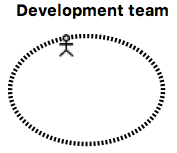
\includegraphics[scale=0.5]{img/actor_development_team} };
        \node[traceNodeRED] (trace1) at (-.5,-.3) {};
        \node[traceNodeRED] (trace2) at (2.2,-0.1) {};

         \path
    (a1) edge[attackLink] (a0)
    (a0) edge [CQLink, bend right=50] node [left,draw=none] {CQ0} (a1)
    (trace1) edge[traceLinkRED] (trace2);
\end{tikzpicture}
\caption{Argument schemes and critical questions (left), GRL model (right), and traceability link (dotted line) of a discussion about the relevance of actor Development team.}
\label{fig:examples:relevant-actor}
\end{figure}

We formalize this using a \emph{generic counterargument}, attacking the critical question. The first part of the discussion is shown in Figure~\ref{fig:examples:relevant-actor}. We formalize the first statement as an instantiation of argument scheme AS0: \texttt{Actor development team is relevant}. This argument is, then, attacked by answering critical question CQ0: \emph{Is actor development team relevant?} with \emph{No}. This results in two arguments, AS0 and CQ0, where CQ0 attacks AS0. This is shown in Figure~\ref{fig:examples:relevant-actor}, left image.

\begin{figure}[ht!]
\centering
        \begin{tikzpicture}
        \node (a0) [argNodeIN] at (-2,0) {
        	\argtext{AS0}{Development team is relevant}
        };
        \node (a1) [argNodeOUT] at (-2,-2.5){
        	\argtext{}{Development team is not relevant (\emph{The professor makes the software})}
        };
        \node (a2) [argNodeIN] at (-2,-5) {
        	\argtext{}{The professor doesn't develop the software}
        } ;
        \node[grl] (actor) at (2.3,-1) { 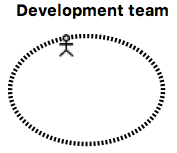
\includegraphics[scale=0.5]{img/actor_development_team} };
        \node[traceNodeGREEN] (trace1) at (-.5,-.3) {};
        \node[traceNodeGREEN] (trace2) at (2.2,-0.1) {};

         \path
    (a1) edge[attackLink] (a0)
    (a2) edge[attackLink] (a1)
    (a0) edge [CQLink, bend right=50] node [left,draw=none] {CQ0} (a1)
    (a1) edge [CQLink, bend right=50] node [left,draw=none] {Att} (a2)
    (trace1) edge[traceLinkGREEN] (trace2);
\end{tikzpicture}
\caption{Argument schemes and critical questions (left), GRL model (right), and traceability link (dotted line) of a discussion about the relevance of actor Development team.}
\label{fig:examples:relevant-actor2}
\end{figure}

Figure~\ref{fig:examples:relevant-actor2} shows the situation after the counter argument has been put forward. The argument ``The professor doesn't develop the software'' now attacks the argument ``\emph{Development team} is not relevant (\emph{The professor makes the software})'', which in turn attacks the original argument ``\emph{Development team} is relevant''. As a result, the first and the last argument are both accepted, which causes the actor in the GRL model to be enabled again.